\chapter{使用方法}
\section{\LaTeX 环境}
本项目宏包依赖\LaTeXe 、Xe\TeX 以及C\TeX ,因此在使用前请确保这些发行版已经安装妥当。
本人在 MacTeX 2015 - Full 在 OS X 10.11 环境下运行通过。文件使用UTF-8编码,并使用 Xe\LaTeX 进行编译。为了方便使用,如果你的操作系统是*nix 环境,那么你可以使用本示例给出的 Makefile 文件执行 make 命令进行文档编译。

\section{目录结构}
项目目录由以下文件构成:
\begin{itemize}
\item \textcolor{blue}{template/*} - 论文宏包及其依赖文件,可以无视这个文件文件夹,我们建议 main.tex 和 此文件夹位于同一目录下,原因是我们不建议你修改应用 SWUNThesis 宏包的方式
\item \textcolor{blue}{main.tex} - 论文的基本骨架,如果 SWUNThesis 不能满足你的要求,那么你可以在此添加你需要的其他宏包,但我们不建议你修改应用 SWUNThesis 宏包的方式
\item \textcolor{blue}{Makefile} - 在*nix(Linux/Mac OS X)环境下,使用 \verb|make| 命令完成论文的整体编译

\item \textcolor{blue}{content/*} - 此文件夹内的文件,包含了论文正文的全部文字信息,其中包括 info.tex 文件中的标题、作者信息等、abstract.tex 文件中的中英文摘要信息、ch*.tex 文件给出的每一章内容等等
\item \textcolor{blue}{data/*} - 此文件夹中给出了论文需要引用到的数据,本宏包支持引用 CSV 文件自动生成展示的表格
\item \textcolor{blue}{figure/*} -  此文件夹中给出了导入图片的示例,本宏包自动增加了对 eps 高清图片的支持
\item \textcolor{blue}{code/main.c} - 此文件夹中包含论文中需要引用到的代码片段,本宏包支持从代码文件中自动引入代码。
\item \textcolor{blue}{references/main.bib} - bibtex 文献库,可以从 GoogleScholar 中获取 BibTex 记录。
\end{itemize}

\section{如何使用}
本文将给予你一个粗略的使用本模版的示例。
\subsection{基本信息}
在 info.tex 文件中输入自己的基本信息。然后论文的摘要可以在 abstract.tex 中输入。同时,英文摘要也可以写在其中。
你可能需要包含自己的宏包,那么你可以在 main.tex 中添加 usepackag 命令。

\subsubsection{多级标题}
另外,随着章节数目增多,可以自行新建 ch*.tex 文件,并将其在 main.tex 中用 include 指令包含进来。最后,为了编译你的论文,你可以使用本示例目录下的 Makefile 文件 直接进行 make。

\section{注意事项}
\begin{enumerate}
\item 中英文摘要不应超过一页,否则第二页的板式会有错误。
\item 所有文件必须是 UTF-8 编码,否则编译不能通过。
\end{enumerate}

\section{插入资源}
这一节内容将向你展示如何插入图片、表格、公式及代码资源。
\subsection{插入图片}
毫无疑问,你肯定需要插入各种各样的图片,下面的图\ref{fig:one}是一个插入图片的例子。

\begin{figure}[htbp!]
\centering
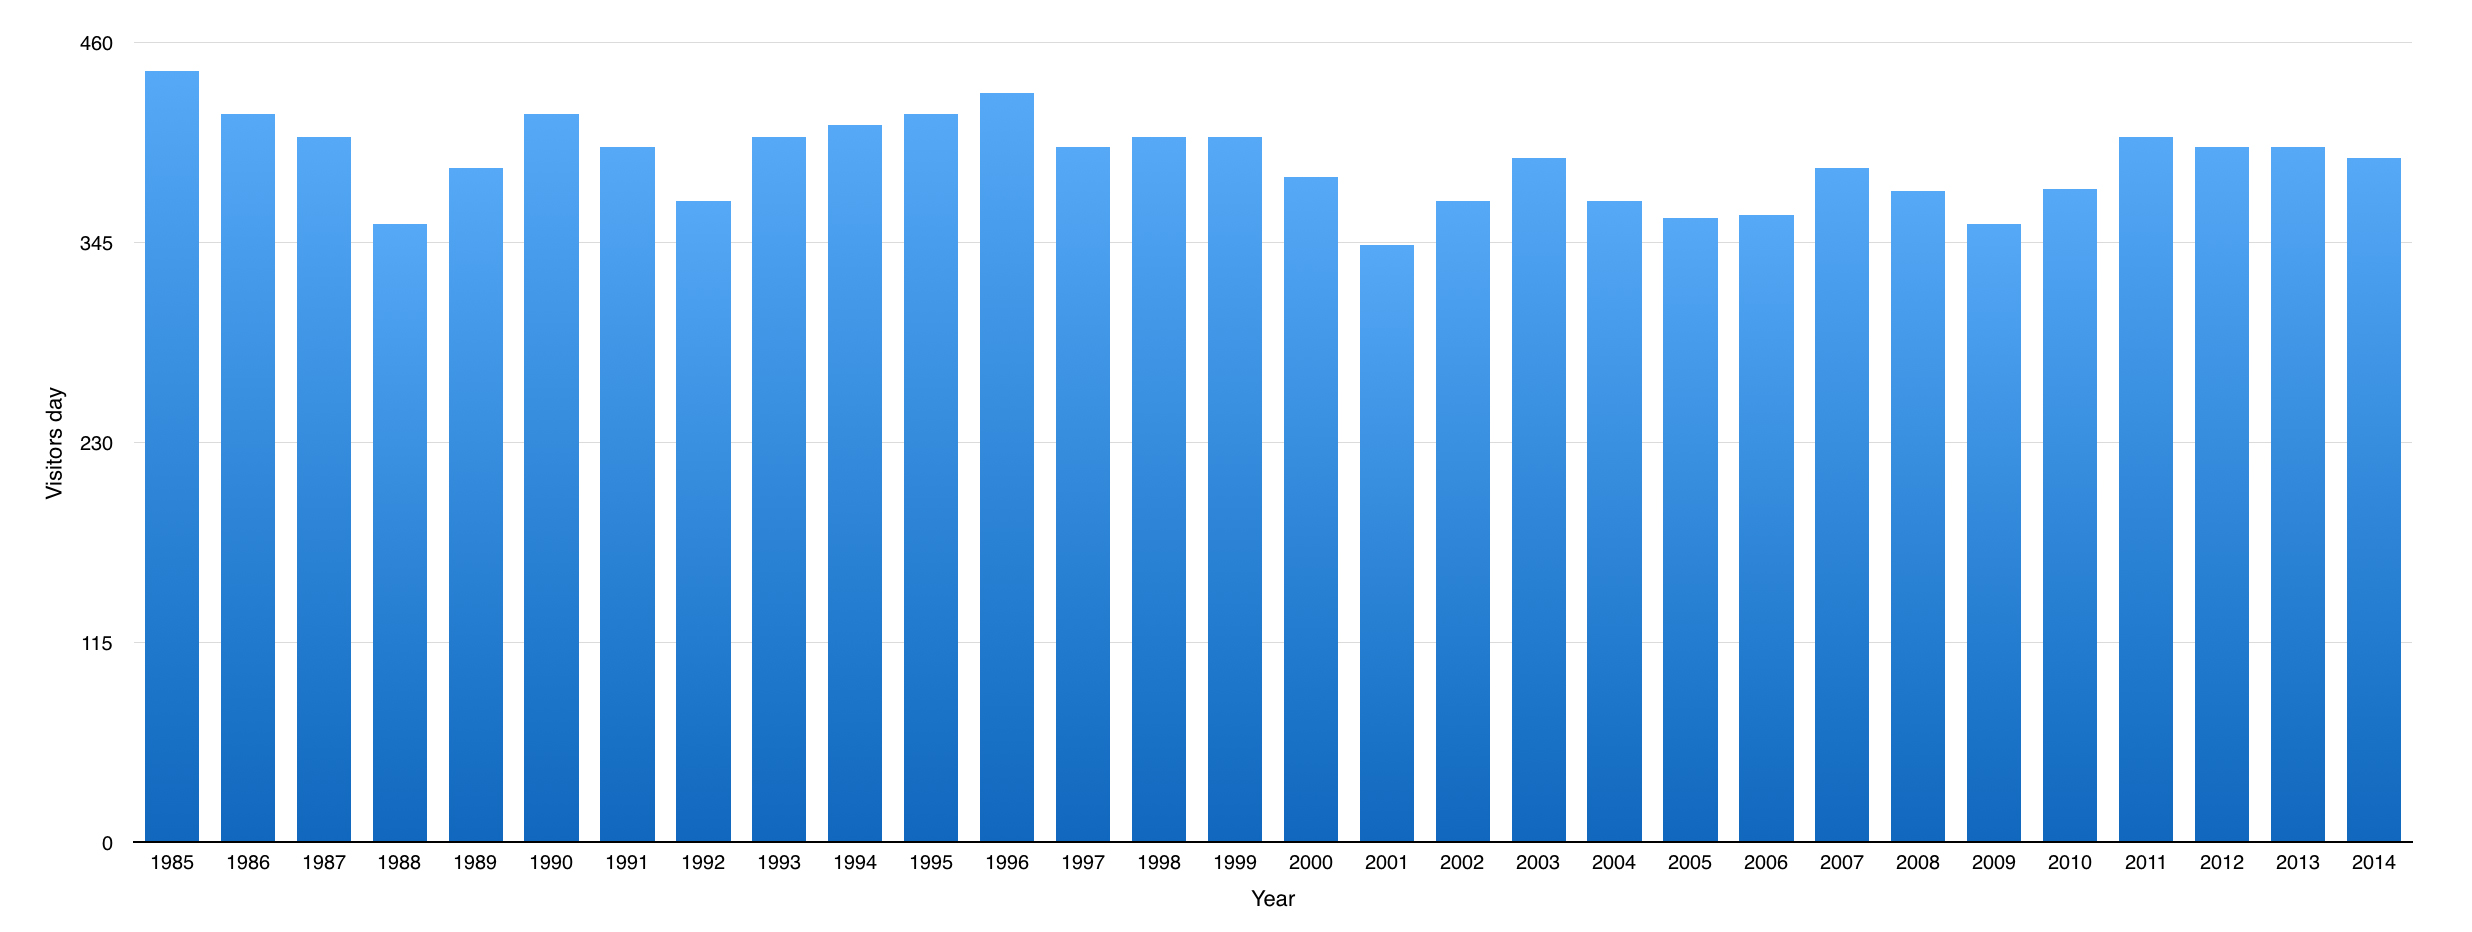
\includegraphics[scale=0.3]{figures/pic.jpg}
\caption{这是一张图片}\label{fig:one}
\end{figure}

当然插入图片你可能还会有其他需求,所以你可以参考一些网上的其他例子,但是就目前这个例子而言已经足够了。

这里插入的是 jpg 格式的图片,在本红包中我们还引入了 eps 图片的支持,你也可以直接引入 eps 图片来获得高精度的显示效果。

\subsection{插入表格}
可能你还需要插入表格,表\ref{table:one}就是一个例子。

\begin{table}[htbp!]
\centering
\caption{这是一张表格}\label{table:one}\par
\csvautobooktabular{data/data.csv}
\end{table}

\subsection{插入公式}

下面则是一个很好的公式混排的例子。

设函数集$Q(z,\alpha ),\alpha \in \Lambda$满足条件

\begin{equation}
A\leq \int_{}^{}Q(z,\alpha ) dF(z)\leq B(A\leq R(\alpha)\leq B),
\end{equation}

那么EMR原则一致性的充分必要条件是:经验风险 $R_{emp}(\alpha)$ 在函数集$ Q(z,\alpha )\in \Lambda $上以如下意义一致收敛于期望风险 $R\left( \alpha \right)$

\begin{equation}
\lim_{l\rightarrow\infty}P \{ \sup_{\alpha\in\Lambda}(R(\alpha)-R_{emp}(\alpha))>\epsilon \}=0,\forall \epsilon>0
\end{equation}

\subsection{插入代码}
如果你是学计算机的,很明显你需要往文章中插入代码,所以,下面的代码展示了如何从文件中插入代码\ref{lst:one}。

\lstinputlisting[
	language={[ANSI]C},
	morekeywords={World},
	emph={printf},
    caption={\kaishu 这段C语言代码的输出结果为 Hello World!},
    label={lst:one}
]{code/main.c}

这里插入的是 C 语言代码,在 \LaTeX 中,除了常见的 C++/Java/HTML/Python/PHP 等等语言外,\LaTeX 的 listings 宏包还支持 SQL/TeX/Haskell/Lisp/R/Matlab/Ruby 等超过 50 种语言,在SWUNThesis 宏包中我们额外增加了对 JavaScript 和 Swift 两个语言的支持,如果你还需求其他的语言,你可以进一步了解。

\subsection{引用文献}

本模板使用 BibTex 管理参考文献,并使用北京邮电大学开发的 BibTex 中文文献管理样式 bstutf8.bst。引用文献可以简单的使用cite 命令进行引用\cite{dongshihai2004, knuth1986texbook}。
